% !TeX root = ../beamer.tex
\section{Signal Korrelation}

\begin{frame}
    \frametitle{Ermittlung der bistatischen Entfernung}

    \begin{itemize}
        \centering
        \item Bestimmung der \textbf{bistatischen Entfernung} aus gemessenem \textbf{Zeitversatz} \(\tau\) zwischen \textbf{Echo-} und \textbf{Referenzsignal}:
              \begin{equation}
                  R = \tau \tikzmarknode{c}{c}
              \end{equation}
              \tikzmarknode{c_txt}{Lichtgeschwindigkeit \(\approx\) \SI[per-mode=symbol]{3e8}{\metre\per\second}}
              \begin{tikzpicture}[remember picture,overlay]
                  \draw [->] (c_txt) to [bend right,in=-100,out=90] (c.south);
              \end{tikzpicture}

              \vspace{\baselineskip}

        \item<2-> \textbf{Wie wird Zeitversatz \(\tau\) gemessen?}
    \end{itemize}
\end{frame}

\begin{frame}
    \frametitle{Referenz- und Echosignal}

    Gepulstes Beispiel:
    \begin{columns}
        \begin{column}{0.5\textwidth}
            \begin{figure}
                \centering
                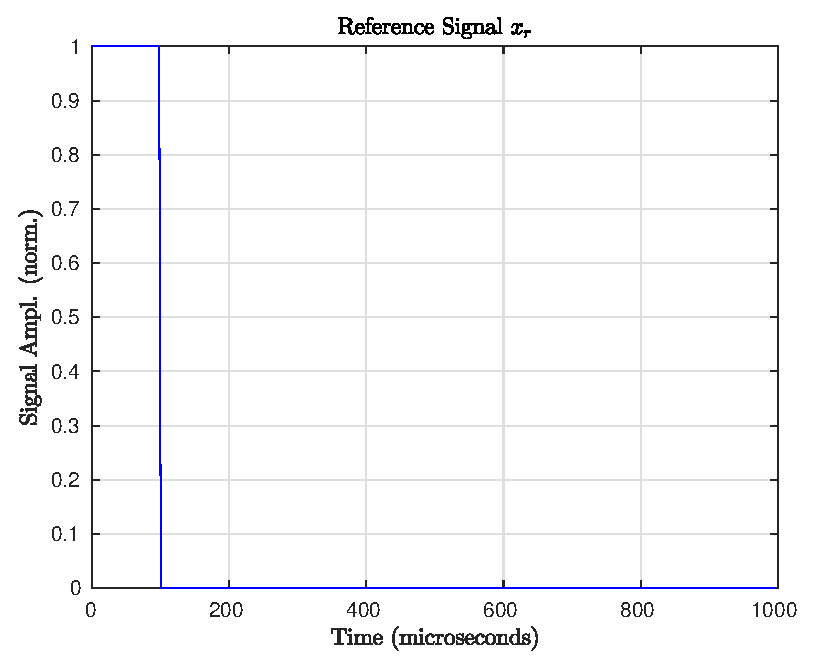
\includegraphics[width=\linewidth,height=\textheight-5\baselineskip,keepaspectratio]{reference_signal.eps}
            \end{figure}
        \end{column}
        \begin{column}{0.5\textwidth}
            \begin{figure}
                \centering
                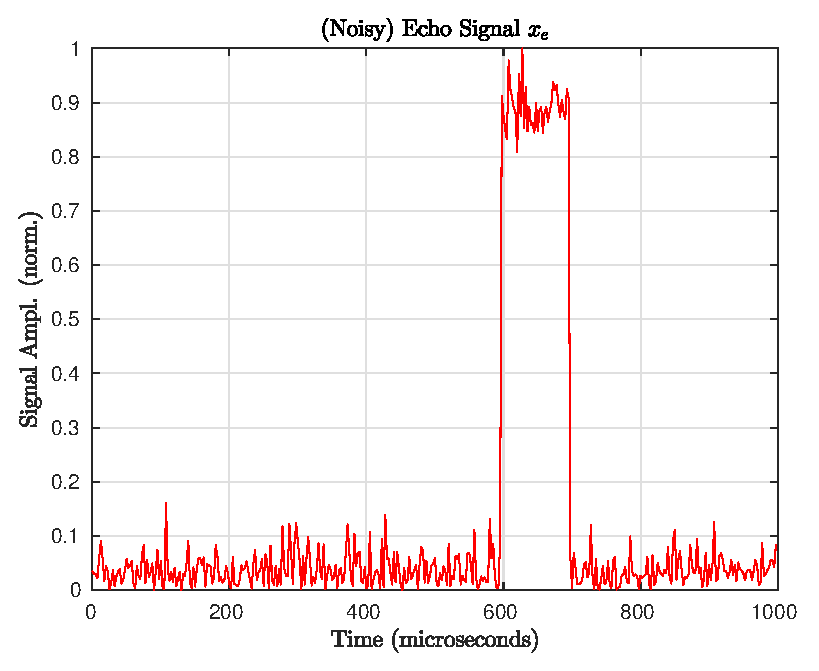
\includegraphics[width=\linewidth,height=\textheight-5\baselineskip,keepaspectratio]{echo_signal.eps}
            \end{figure}
        \end{column}
    \end{columns}
\end{frame}

\begin{frame}
    \frametitle{Kreuzkorrelation}

    \begin{figure}
        \centering
        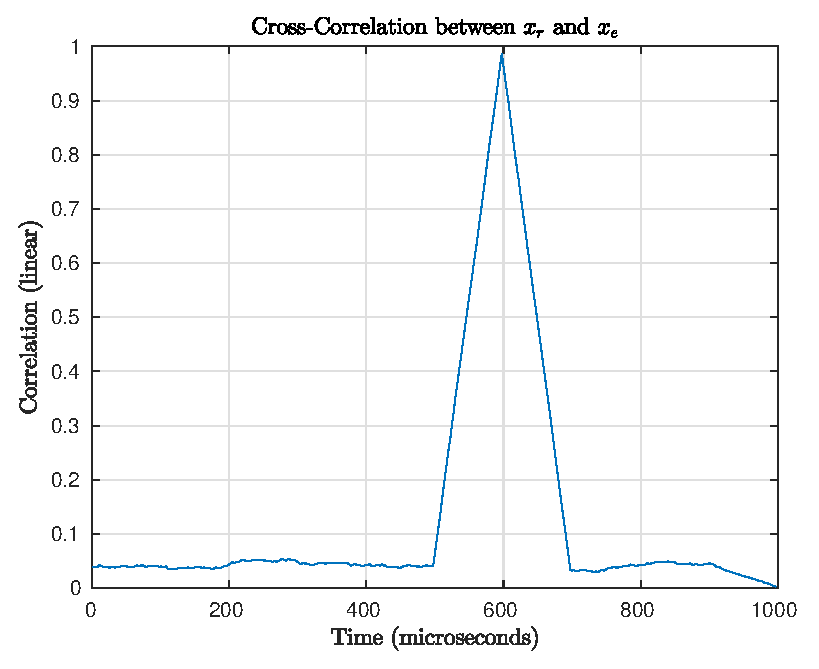
\includegraphics[width=\linewidth,height=\textheight-3\baselineskip,keepaspectratio]{correlation_linear.eps}
    \end{figure}
\end{frame}

\begin{frame}
    \frametitle{Kreuzkorrelation}

    \begin{itemize}
        \item Gibt Aussage über \textbf{Zeitversatz} zweier Signale
        \item Definition für Referenzsignal \(x_{r}\) und Echosignal \(x_{e}\):
              \begin{equation}
                  \psi(t) = \int_{-T/2}^{T/2}{ x_{e}(s) x_{r}^{*}(s - t) \, d s}
              \end{equation}
        \item<2-> Ausgedrückt als bistatische Entfernung (\(R = c t\)):
              \begin{equation}
                  \psi(R) = \int_{-T/2}^{T/2}{ x_{e}(s) x_{r}^{*} \left( s - \frac{R}{c} \right) \, d s}
              \end{equation}
        \item<3-> Wird über \textbf{Bereich von \(R\)} ausgewertet
    \end{itemize}
\end{frame}

\begin{frame}
    \frametitle{Nächster Schritt: Kreuzambiguitätsfunktion}

    \begin{itemize}
        \item Definition:
              \begin{equation}
                  \psi(R, V) = \int_{-T/2}^{T/2} {x_{e}(s) \cdot x_{r}^{*}} \left( s - \frac{R}{c} \right)\mathrm{e}^{- \mathrm{j} \frac{2 \pi}{\lambda} V s} \, d s
              \end{equation}
        \item Berücksichtigt auch \textbf{Dopplershift} und damit bistatische Geschw.
        \item Wird über \textbf{Bereich von \(R\) und \(V\)} ausgewertet
    \end{itemize}
\end{frame}

\begin{frame}
    \frametitle{Range-Doppler Map}

    \begin{figure}
        \centering
        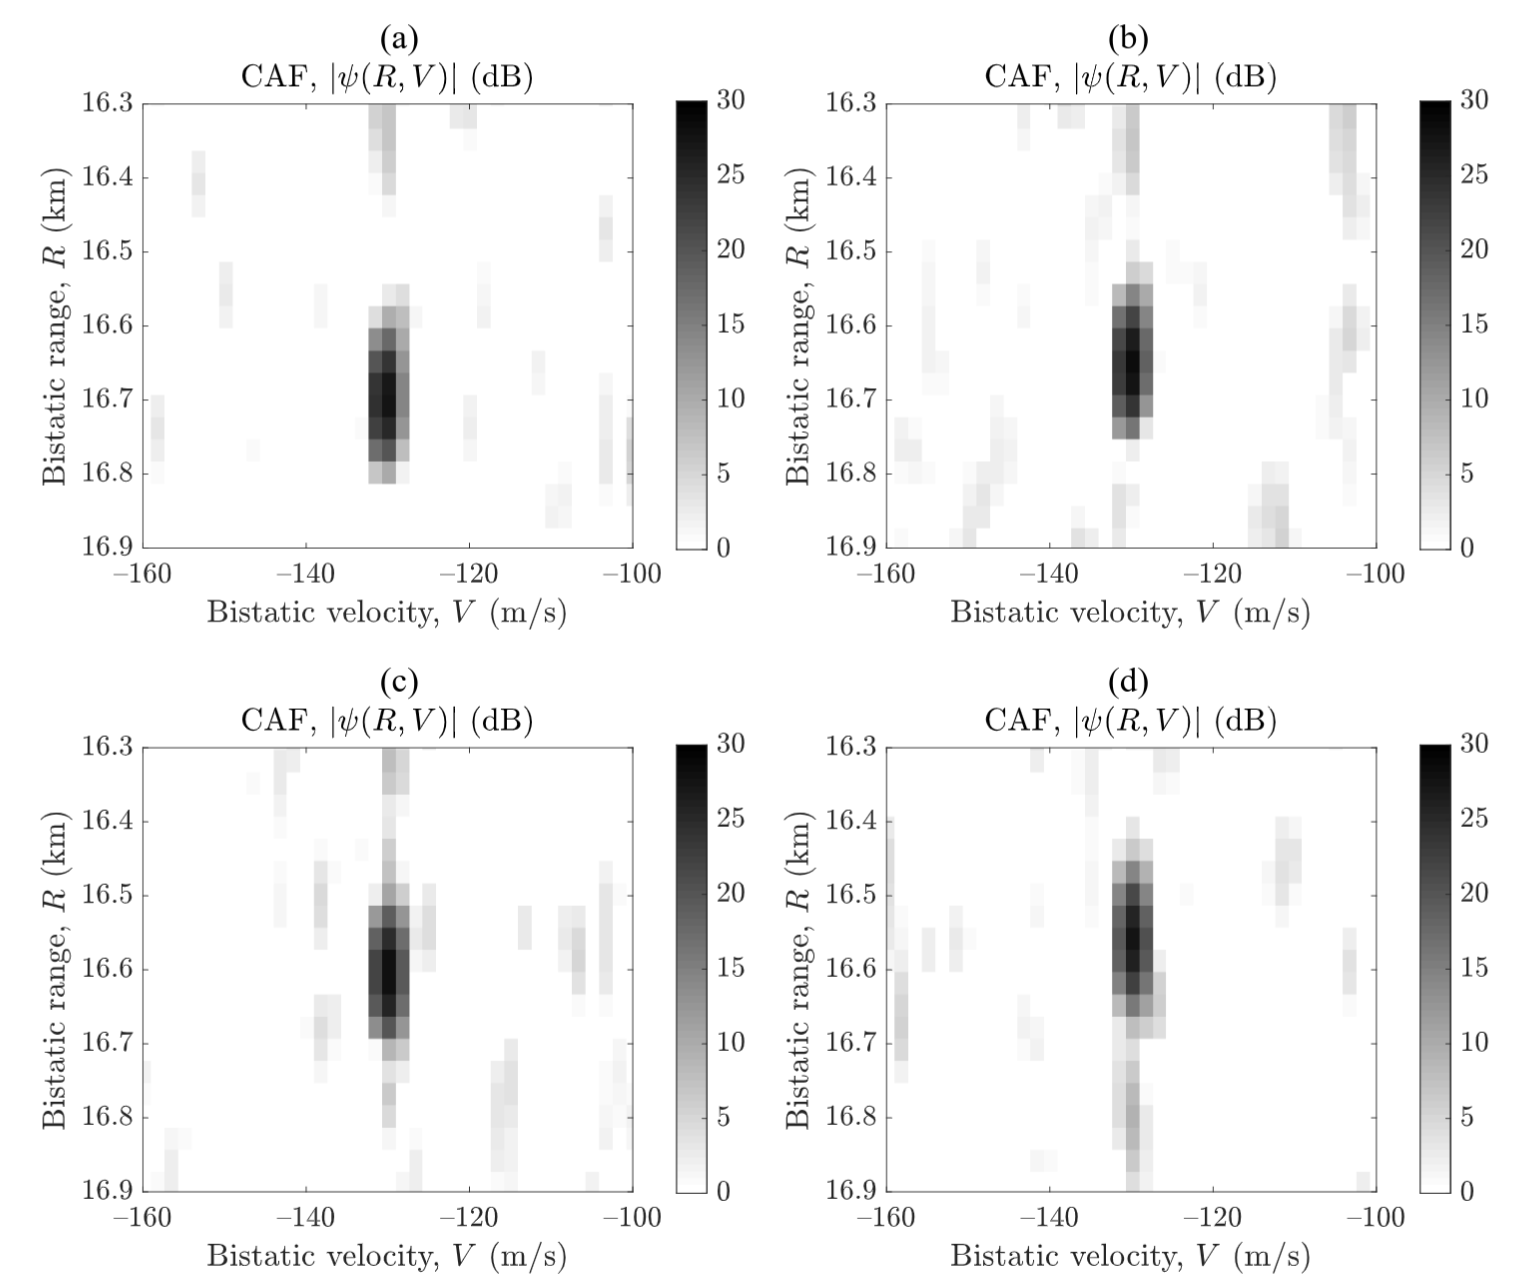
\includegraphics[width=\linewidth,height=\textheight-5\baselineskip,keepaspectratio]{range_doppler.png}
        \caption{Ausschnitt aus Kreuzambiguitätsfunktion für bewegtes Ziel~\cite[p.~161]{Malanowski2019}.}
    \end{figure}
\end{frame}

\begin{frame}
    \frametitle{Transformation in Kartesische Koordinaten}

    \Large Wie gelangt man von \textbf{bistatischer} zur \textbf{kartesischen Darstellung}?\normalsize

    \vspace{2\baselineskip}

    Möglichkeiten:
    \begin{enumerate}
        \item \textbf{Antennenrichtwirkung} nutzen um bistatischen Ellipsoiden \emph{abzutasten}
        \item \textbf{Ellipsoiden} verschiedener Rx-Tx Paare \textbf{übereinanderlegen}
    \end{enumerate}
\end{frame}


\begin{frame}
    \frametitle{Schnittpunkte der bistatischen Ellipse}

    \begin{figure}
        \centering
        \begin{adjustbox}{max width=\linewidth,totalheight=\textheight-5\baselineskip}
            \begin{tikzpicture}
                
\def\F{5}
\coordinate (rx1_coord) at (-\F,0);
\coordinate (tx1_coord) at (\F,0);
\coordinate (tx2_coord) at (2,2);
\coordinate (tx3_coord) at (1,-3);
\coordinate (target_coord) at (2,3.5);

\draw [visible on=<2->]
let
\p1=(tx1_coord),
\p2=($(target_coord)-(\p1)$),
\p3=($(target_coord)-(rx1_coord)$),
\p4=($(\p1)-(rx1_coord)$),
\n1={scalar((veclen(\x2,\y2) + veclen(\x3,\y3))*1pt/1cm)},
\n2={scalar(veclen(\x4,\y4)*1pt/1cm)},
\n3={sqrt(pow(\n1/2, 2))},
\n4={sqrt(pow(\n1/2, 2) - pow(\n2/2, 2))},
in
($(rx1_coord)!0.5!(\p1)$)
circle [x radius=\n3,y radius=\n4,draw=gray];

\draw [visible on=<3->]
let
\p1=(tx2_coord),
\p2=($(target_coord)-(\p1)$),
\p3=($(target_coord)-(rx1_coord)$),
\p4=($(\p1)-(rx1_coord)$),
\n1={scalar((veclen(\x2,\y2) + veclen(\x3,\y3))*1pt/1cm)},
\n2={scalar(veclen(\x4,\y4)*1pt/1cm)},
\n3={sqrt(pow(\n1/2, 2))},
\n4={sqrt(pow(\n1/2, 2) - pow(\n2/2, 2))},
in
($(rx1_coord)!0.5!(\p1)$)
circle [x radius=\n3,y radius=\n4,draw=gray,rotate=15.94];

\draw [visible on=<4->]
let
\p1=(tx3_coord),
\p2=($(target_coord)-(\p1)$),
\p3=($(target_coord)-(rx1_coord)$),
\p4=($(\p1)-(rx1_coord)$),
\n1={scalar((veclen(\x2,\y2) + veclen(\x3,\y3))*1pt/1cm)},
\n2={scalar(veclen(\x4,\y4)*1pt/1cm)},
\n3={sqrt(pow(\n1/2, 2))},
\n4={sqrt(pow(\n1/2, 2) - pow(\n2/2, 2))},
in
($(rx1_coord)!0.5!(\p1)$)
circle [x radius=\n3,y radius=\n4,draw=gray,rotate=-26.57];

\draw [dotted] (rx1_coord) node [cross out,draw,solid] {} node [below=2pt] {Rx}  -- (tx1_coord) node [cross out,draw,solid] {} node [below=2pt] {Tx1};

\draw [dotted] (rx1_coord) -- (tx2_coord) node [cross out,draw,solid] {} node [below=2pt] {Tx2};
\draw [dotted] (rx1_coord) -- (tx3_coord) node [cross out,draw,solid] {} node [below=2pt] {Tx3};

\node at (target_coord) [visible on=<1>] {\faPlane};
\node at (target_coord) [visible on=<4>] {\faPlane};

            \end{tikzpicture}
        \end{adjustbox}
        \caption{Schnittpunktmethode}
    \end{figure}
\end{frame}
